%=======================================================
% CHAPTER 1: LINEAR CODES
%=======================================================

\begin{frame}[plain]
  \begin{center}\bfseries\centering
    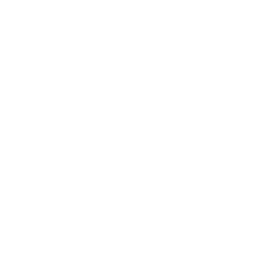
\includegraphics[scale=1]{assets/branding/opa0}
    \vspace{-5.75cm}\\
    {\adjustbox{scale=2.15}{\color{TealDarkCyan}\;II.\;Linear Codes}}
    \bigskip\bigskip
    {\ }\vspace{4cm}\\
    \bigskip
  \end{center}
\end{frame}

\begin{frame}{\textbf{II. Linear Codes}}{The ambient space}
\small
\defbox[Hamming space]{
Fix a finite field $\F_q$. The set $\F_q^n$ is simultaneously a vector space and a metric space with
\[
  d(x,y)=\#\{i:x_i\ne y_i\}.
\]
}
\begin{itemize}
  \item The metric is translation invariant: $d(x+z,y+z)=d(x,y)$.
  \item The spheres are combinatorial objects:
  \[
    |B_t(0)|=\sum_{i=0}^t \binom{n}{i}(q-1)^i.
  \]
  \item Coding theory asks for large subsets with large mutual distance.
\end{itemize}
\end{frame}

\begin{frame}{\textbf{II. Linear Codes}}{Codes as metric subsets}
\small
\defbox[Code]{
A code of length $n$ over $\F_q$ is a subset $\code\subseteq \F_q^n$. Its minimum distance is
\[
  d(\code)=\min\{d(x,y):x,y\in\code,\ x\ne y\}.
\]
}
\begin{block}{Mathematician's viewpoint}
The fundamental problem is an extremal problem in a finite metric space:
\[
  A_q(n,d)=\max\{|\code|:\code\subseteq\F_q^n,\ d(\code)\ge d\}.
\]
\end{block}
\end{frame}

\begin{frame}{\textbf{II. Linear Codes}}{Linearity}
\small
\defbox[Linear code]{
A linear $[n,k,d]_q$ code is a $k$-dimensional subspace
\[
  \code\le \F_q^n
\]
with minimum distance $d$.
}
\begin{itemize}
  \item The cardinality is forced: $|\code|=q^k$.
  \item The rate is $R=k/n$.
  \item Since $\code$ is a group under addition,
  \[
    d(\code)=\min\{\wt(c):0\ne c\in\code\}.
  \]
\end{itemize}
\end{frame}

\begin{frame}{\textbf{II. Linear Codes}}{Weight}
\small
\defbox[Hamming weight]{
For $x=(x_1,\ldots,x_n)\in\F_q^n$,
\[
  \wt(x)=|\supp(x)|,\qquad \supp(x)=\{i:x_i\ne0\}.
\]
}
\begin{block}{Lemma}
For a linear code $\code$,
\[
  d(\code)=\min_{0\ne c\in\code}\wt(c).
\]
\end{block}
\textbf{Proof.} If $x,y\in\code$, then $x-y\in\code$ and $d(x,y)=\wt(x-y)$.
\end{frame}

\begin{frame}{\textbf{II. Linear Codes}}{Generator matrices}
\small
\defbox[Generator matrix]{
A generator matrix for an $[n,k]_q$ code is a matrix $G\in\F_q^{k\times n}$ whose rows form a basis of $\code$.
Encoding is the linear map
\[
  \F_q^k\longrightarrow \F_q^n,\qquad m\longmapsto mG.
\]
}
\begin{itemize}
  \item The code is the row space of $G$.
  \item Different bases give different generator matrices for the same code.
  \item Replacing $G$ by $UG$, $U\in\operatorname{GL}_k(\F_q)$, changes coordinates on messages only.
\end{itemize}
\end{frame}

\begin{frame}{\textbf{II. Linear Codes}}{Equivalence of descriptions}
\small
\thmbox[Row-space equivalence]{
Two full-rank matrices $G,G'\in\F_q^{k\times n}$ generate the same code if and only if
\[
  G'=UG
\]
for some $U\in\operatorname{GL}_k(\F_q)$.
}
\begin{itemize}
  \item This is just change of basis in the subspace $\code$.
  \item The code is the invariant object; the matrix is a coordinate choice.
  \item Many computational algorithms are Gaussian elimination on this statement.
\end{itemize}
\end{frame}

\begin{frame}{\textbf{II. Linear Codes}}{Systematic form}
\small
\defbox[Systematic generator matrix]{
After permuting coordinates, many generator matrices can be written
\[
  G=[I_k\mid P].
\]
}
\begin{itemize}
  \item The message appears visibly in the first $k$ coordinates.
  \item The remaining $n-k$ coordinates are parity symbols.
  \item Systematic form is convenient, but it is not an intrinsic property of the code.
\end{itemize}
\begin{block}{Caution}
Coordinate permutations preserve distance, but they change the visible positions of message and parity symbols.
\end{block}
\end{frame}

\begin{frame}{\textbf{II. Linear Codes}}{Parity-check matrices}
\small
\defbox[Parity-check matrix]{
A parity-check matrix is a matrix $H\in\F_q^{(n-k)\times n}$ such that
\[
  \code=\ker(H)=\{c\in\F_q^n:Hc^T=0\}.
\]
}
\begin{itemize}
  \item If $G$ generates $\code$, then $GH^T=0$.
  \item The rows of $H$ generate the dual code $\code^\perp$.
  \item The equation $Hc^T=0$ is a system of homogeneous parity constraints.
\end{itemize}
\end{frame}

\begin{frame}{\textbf{II. Linear Codes}}{Duality}
\small
\defbox[Dual code]{
The dual of $\code\le\F_q^n$ is
\[
  \code^\perp=\{y\in\F_q^n:\langle x,y\rangle=0\text{ for all }x\in\code\}.
\]
}
\begin{block}{Dimension identity}
\[
  \dim\code+\dim\code^\perp=n.
\]
\end{block}
\begin{itemize}
  \item A parity-check matrix for $\code$ is a generator matrix for $\code^\perp$.
  \item Duality exchanges constraints and codewords.
\end{itemize}
\end{frame}

\begin{frame}{\textbf{II. Linear Codes}}{Distance from checks}
\small
\thmbox[Column criterion]{
Let $H$ be a parity-check matrix of $\code$. Then $d(\code)$ is the least number of columns of $H$ that are linearly dependent.
}
\begin{proof}
A vector $c$ of weight $s$ satisfies $Hc^T=0$ exactly when a linear combination of the $s$ corresponding columns is zero.
\end{proof}
\begin{itemize}
  \item No zero column means $d\ge2$.
  \item No proportional columns means $d\ge3$.
  \item This criterion is the entrance to Hamming codes.
\end{itemize}
\end{frame}

\begin{frame}{\textbf{II. Linear Codes}}{Syndromes}
\small
\defbox[Syndrome]{
For a received word $v=c+e$, define
\[
  s(v)=Hv^T.
\]
Since $Hc^T=0$, one has
\[
  s(v)=He^T.
\]
}
\begin{itemize}
  \item The syndrome depends only on the error coset.
  \item $s(v)=0$ if and only if $v\in\code$.
  \item Decoding is the problem of choosing a likely error in each coset.
\end{itemize}
\end{frame}

\begin{frame}{\textbf{II. Linear Codes}}{Cosets}
\small
\defbox[Coset decomposition]{
The ambient space is a disjoint union of cosets:
\[
  \F_q^n=\coprod_{a\in A}(a+\code),
\]
where $|A|=q^{n-k}$.
}
\begin{itemize}
  \item All words in the same coset have the same syndrome.
  \item Syndromes parameterize cosets when $H$ has full rank.
  \item Decoding assigns to each coset a chosen representative of small weight.
\end{itemize}
\end{frame}

\begin{frame}{\textbf{II. Linear Codes}}{Standard arrays}
\small
\defbox[Coset leader]{
A coset leader is an element of least Hamming weight in a coset $a+\code$.
}
\begin{itemize}
  \item The standard array lists cosets by their leaders.
  \item Nearest-neighbor decoding subtracts the coset leader.
  \item The method is conceptually clean but exponential in $n-k$.
\end{itemize}
\begin{block}{Principle}
Good algebraic families replace the standard array by structure.
\end{block}
\end{frame}

\begin{frame}{\textbf{II. Linear Codes}}{Correction and detection}
\small
\thmbox[Distance theorem]{
A code of minimum distance $d$ detects every error of weight at most $d-1$ and corrects every error of weight at most
\[
  t=\left\lfloor\frac{d-1}{2}\right\rfloor.
\]
}
\begin{itemize}
  \item Detection: no nonzero error of weight $<d$ is a codeword.
  \item Correction: balls of radius $t$ around distinct codewords are disjoint.
\end{itemize}
\end{frame}

\begin{frame}{\textbf{II. Linear Codes}}{Packing}
\small
\thmbox[Hamming bound]{
If $\code$ is an $[n,k,d]_q$ code and $t=\lfloor(d-1)/2\rfloor$, then
\[
  q^k\sum_{i=0}^t \binom{n}{i}(q-1)^i\le q^n.
\]
}
\begin{proof}
The balls of radius $t$ around codewords are disjoint subsets of $\F_q^n$.
\end{proof}
\begin{block}{Perfect code}
Equality means the radius-$t$ balls tile the whole Hamming space.
\end{block}
\end{frame}

\begin{frame}{\textbf{II. Linear Codes}}{Singleton bound}
\small
\thmbox[Singleton bound]{
Every $[n,k,d]_q$ code satisfies
\[
  d\le n-k+1.
\]
}
\begin{proof}
Delete $d-1$ coordinates. Distinct codewords must remain distinct, so $q^k\le q^{n-d+1}$.
\end{proof}
\begin{itemize}
  \item Codes meeting the bound are called MDS codes.
  \item Reed--Solomon codes are the standard nonbinary MDS examples.
\end{itemize}
\end{frame}

\begin{frame}{\textbf{II. Linear Codes}}{Gilbert--Varshamov idea}
\small
\thmbox[Existence principle]{
There exist linear codes whose parameters are good because a greedy construction cannot cover the whole space too early.
}
\[
  q^k\sum_{i=0}^{d-2}\binom{n-1}{i}(q-1)^i < q^n
  \quad\Rightarrow\quad
  \text{an }[n,k,d]_q\text{ code exists.}
\]
\begin{itemize}
  \item This is not a construction one wants to implement.
  \item It proves that the asymptotic landscape is nontrivial.
  \item Algebraic families try to approach such existence bounds explicitly.
\end{itemize}
\end{frame}

\begin{frame}{\textbf{II. Linear Codes}}{Griesmer bound}
\small
\thmbox[Griesmer bound]{
For a linear $[n,k,d]_q$ code,
\[
  n\ge \sum_{i=0}^{k-1}\left\lceil \frac{d}{q^i}\right\rceil.
\]
}
\begin{itemize}
  \item This is stronger than Singleton in many small-parameter cases.
  \item It comes from repeatedly puncturing on the support of a minimum word.
  \item It is a linear-code bound: linearity is essential.
\end{itemize}
\end{frame}

\begin{frame}{\textbf{II. Linear Codes}}{Puncturing}
\small
\defbox[Puncturing]{
Puncturing a code at coordinate $i$ means deleting the $i$-th coordinate from every word.
}
\begin{itemize}
  \item Length decreases by one.
  \item Dimension usually stays the same, but can drop.
  \item Minimum distance can decrease by at most one.
\end{itemize}
\begin{block}{Use}
Puncturing is the basic operation for inductive arguments on code parameters.
\end{block}
\end{frame}

\begin{frame}{\textbf{II. Linear Codes}}{Shortening}
\small
\defbox[Shortening]{
Shortening at coordinate $i$ means first selecting codewords with $c_i=0$, then puncturing at $i$.
}
\begin{itemize}
  \item Length decreases by one.
  \item Dimension can decrease by one.
  \item Minimum distance does not decrease.
\end{itemize}
\begin{block}{Duality}
Puncturing and shortening are dual operations:
\[
  (\text{puncture } \code)^\perp=\text{shorten }(\code^\perp).
\]
\end{block}
\end{frame}

\begin{frame}{\textbf{II. Linear Codes}}{Weight enumerators}
\small
\defbox[Weight enumerator]{
The weight enumerator is
\[
  W_\code(X,Y)=\sum_{c\in\code}X^{n-\wt(c)}Y^{\wt(c)}.
\]
}
\begin{itemize}
  \item It records the distribution of weights.
  \item The minimum distance is the first nonzero exponent of $Y$ after the constant term.
  \item It is a coarser invariant than the code but a powerful one.
\end{itemize}
\end{frame}

\begin{frame}{\textbf{II. Linear Codes}}{MacWilliams identity}
\small
\thmbox[MacWilliams identity]{
For a linear $[n,k]_q$ code,
\[
  W_{\code^\perp}(X,Y)=\frac{1}{|\code|}W_\code(X+(q-1)Y,X-Y).
\]
}
\begin{itemize}
  \item The identity is a finite Fourier transform.
  \item It turns the weight distribution of $\code$ into that of $\code^\perp$.
  \item It is one of the central reasons duality is computationally useful.
\end{itemize}
\end{frame}

\begin{frame}{\textbf{II. Linear Codes}}{Self-orthogonality}
\small
\defbox[Self-orthogonal and self-dual]{
A code is self-orthogonal if $\code\subseteq\code^\perp$ and self-dual if $\code=\code^\perp$.
}
\begin{itemize}
  \item Self-dual binary codes have dimension $n/2$.
  \item Doubly-even self-dual codes have all weights divisible by $4$.
  \item Such codes connect coding theory to lattices and modular forms.
\end{itemize}
\end{frame}

\begin{frame}{\textbf{II. Linear Codes}}{Equivalent codes}
\small
\defbox[Monomial equivalence]{
Two $q$-ary linear codes are equivalent if one is obtained from the other by permuting coordinates and multiplying coordinates by nonzero scalars.
}
\begin{itemize}
  \item Over $\F_2$, this is just coordinate permutation.
  \item Equivalent codes have the same parameters and weight enumerator.
  \item Classification means classification up to this equivalence.
\end{itemize}
\end{frame}

\begin{frame}{\textbf{II. Linear Codes}}{Automorphisms}
\small
\defbox[Automorphism group]{
\[
  \Aut(\code)=\{\pi\in S_n:\pi(\code)=\code\}
\]
in the binary case.
}
\begin{itemize}
  \item A large automorphism group is a sign of hidden geometry.
  \item Symmetry reduces decoding complexity.
  \item Hamming and cyclic codes both arise from strong symmetry.
\end{itemize}
\end{frame}

\begin{frame}{\textbf{II. Linear Codes}}{Repetition code}
\small
\defbox[Repetition code]{
\[
  \code=\{(a,a,\ldots,a):a\in\F_q\}
\]
is an $[n,1,n]_q$ code.
}
\begin{itemize}
  \item It has maximal distance for dimension $1$.
  \item Its rate is $1/n$, so it is inefficient.
  \item It corrects $\lfloor(n-1)/2\rfloor$ errors by majority vote when $q=2$.
\end{itemize}
\end{frame}

\begin{frame}{\textbf{II. Linear Codes}}{Single parity-check code}
\small
\defbox[Parity-check code]{
\[
  \code=\{x\in\F_q^n:x_1+\cdots+x_n=0\}
\]
is an $[n,n-1,2]_q$ code.
}
\begin{itemize}
  \item The parity-check matrix is $H=[1\;1\;\cdots\;1]$.
  \item It detects one error but cannot correct one error.
  \item It is the dual of the repetition code.
\end{itemize}
\end{frame}

\begin{frame}{\textbf{II. Linear Codes}}{The simplex code}
\small
\defbox[Binary simplex code]{
Let $H_r$ be the matrix whose columns are all nonzero vectors of $\F_2^r$. The row space of $H_r$ is the simplex code.
}
\begin{itemize}
  \item It has parameters $[2^r-1,r,2^{r-1}]_2$.
  \item Every nonzero codeword has the same weight.
  \item Its dual is the binary Hamming code.
\end{itemize}
\end{frame}

\begin{frame}{\textbf{II. Linear Codes}}{Matroid viewpoint}
\small
\defbox[Vector matroid of a code]{
A parity-check matrix $H$ defines a matroid on the coordinate set $\{1,\ldots,n\}$ by linear dependence of columns.
}
\begin{itemize}
  \item Circuits of the matroid correspond to minimal support codewords.
  \item The minimum distance is the size of the smallest circuit.
  \item Projective geometry enters when the columns of $H$ are projective points.
\end{itemize}
\end{frame}

\begin{frame}{\textbf{II. Linear Codes}}{Tanner graphs}
\small
\defbox[Tanner graph]{
Given a parity-check matrix $H$, form a bipartite graph with variable nodes $1,\ldots,n$ and check nodes equal to the rows of $H$.
}
\begin{itemize}
  \item An edge joins variable $j$ to check $i$ when $H_{ij}\ne0$.
  \item Sparse $H$ gives iterative decoding algorithms.
  \item Classical algebraic codes often have dense checks; LDPC codes emphasize sparsity.
\end{itemize}
\end{frame}

\begin{frame}{\textbf{II. Linear Codes}}{Decoding hardness}
\small
\thmbox[Syndrome decoding problem]{
Given $H$, a syndrome $s$, and an integer $t$, decide whether there exists $e$ with
\[
  He^T=s,\qquad \wt(e)\le t.
\]
}
\begin{itemize}
  \item This problem is NP-complete in general.
  \item Code-based cryptography is built around this hardness.
  \item Algebraic code families are useful because they add trapdoor-like structure.
\end{itemize}
\end{frame}

\begin{frame}{\textbf{II. Linear Codes}}{Perfect codes}
\small
\defbox[Perfect code]{
A code correcting $t$ errors is perfect if the radius-$t$ balls around codewords partition $\F_q^n$.
}
\[
  |\code|\sum_{i=0}^t \binom{n}{i}(q-1)^i=q^n.
\]
\begin{itemize}
  \item Perfect codes are extremely rare.
  \item The binary Hamming codes are perfect one-error-correcting codes.
  \item The Golay codes are the exceptional perfect codes.
\end{itemize}
\end{frame}

\begin{frame}{\textbf{II. Linear Codes}}{Why linear codes are central}
\small
\begin{columns}[T,onlytextwidth]
  \begin{column}{.48\textwidth}
    \defbox[Algebra]{
    \begin{itemize}\small
      \item subspaces
      \item duality
      \item matrices
      \item finite fields
    \end{itemize}
    }
  \end{column}
  \begin{column}{.48\textwidth}
    \defbox[Algorithms]{
    \begin{itemize}\small
      \item encoding by $G$
      \item checking by $H$
      \item syndrome decoding
      \item structured families
    \end{itemize}
    }
  \end{column}
\end{columns}
\end{frame}

\begin{frame}{\textbf{II. Linear Codes}}{The road to Hamming}
\small
\begin{block}{Question}
Can we construct a linear code that corrects one error and wastes no syndrome?
\end{block}
\begin{itemize}
  \item One error at one of $n$ positions gives $n$ possibilities.
  \item No error gives one more possibility.
  \item A parity-check matrix with $r$ rows has $2^r$ binary syndromes.
\end{itemize}
\[
  n+1=2^r
\]
is the numerology of binary Hamming codes.
\end{frame}
